\documentclass{article}
\setlength\parindent{0pt}
% Language setting
% Replace `english' with e.g. `spanish' to change the document language
\usepackage[english]{babel}
\usepackage{float} % idk what this is for. doc breaks without it
\usepackage{subfig} %for side-by-side image

% Set page size and margins
% Replace `letterpaper' with `a4paper' for UK/EU standard size
\usepackage[letterpaper,top=2cm,bottom=2cm,left=3cm,right=3cm,marginparwidth=1.75cm]{geometry}

% Useful packages
\usepackage{amsmath}
\usepackage{graphicx}
\usepackage[colorlinks=true, allcolors=blue]{hyperref}

\title{MTHM506 Statistical Data Modelling Group Project}
\author{Group 2}

\begin{document}
\maketitle

\section{Introduction}

\subsection{Problem Statement}

Conduct an analysis of tuberculosis (TB) data originating from Brazil, using Generalized
Additive Models (GAMs). Brazil is divided into 557 administrative microregions and the available data
comprises of counts of TB cases in each microregion for each of the years 2012-2014.
\newline

\subsection{Exploration of the problem and the data}

The data is investigated for correlations as these may interfere with later inference from the model(s). Covariates with the highest correlations are - Illiteracy, Poverty, Poor Sanitation and Urbanisation (see: Figure \ref{fig:pearson_correl}). Further tests show which terms should not be considered in a model.
\newline

\section{The Model}	

We want to model the count of cases $TB_i$ by actually modelling $\rho_i$ using
$$
\begin{aligned}
TB_i \sim Pois(\lambda_i = z_i \rho_i) \ TB_i\  \mathrm{indep.} 
\\
log(\lambda_i) = log(z_i) + log(\rho_i)
\end{aligned}
$$
where $TB_i$ is the count of TB cases, $z_i$ is the total population. Model $log(\rho_i)$ as

$$
\begin{aligned}
log(\rho_i) = \sum_{j=1}^{8}f_{j}(x_{i,j})
\\
f(x_i) = \sum_{k=1}^{q}\beta_{k}b_{k}(x_i)
\end{aligned}
$$
where $x_{i,j}$ is the $j$th covariate (out of 8 socio-economic covariates) for the $i$th instance/datum in the dataset and $f(\cdot)$ is a smooth function of said covariate. Hence, the model boils down to
$$
\begin{aligned}
TB_i \sim Pois(\lambda_i = z_i \rho_i) \ TB_i\  \mathrm{indep.} 
\\
log(\lambda_i) = log(z_i) +  \sum_{j=1}^{8}\sum_{k=1}^{q}\beta_{j,k}b_{j,k}(x_{i,j})
\end{aligned}
$$

Looking at the distribution of the residuals of the model, we can see that the data is clearly far too overdispersed to be modelled by a Poisson, which has a fixed dispersion parameter. Even with 80 knots per smooth term the model doesn't seem to have enough flexibility which may be another indicator that a Poisson model is unsuitable for such overdispersed data. We propose the conventional alternative to the Poisson - the Negative Binomial model. Doing so, leads to a drop in the AIC. So the model distribution is changed to Negative Binomial with the same parameterisation except for
the feature that the count of TB cases is now Negative Binomial distributed with mean as described above.
See Table \ref{tab:widgets} appendix for a showcase of different model configurations and their associated AIC.
$$
\begin{aligned}
TB_i \sim NB(\lambda_i , \sigma_i^2) \ TB_i\  \mathrm{indep.} 
\\
\lambda_i = z_i \rho_i ;\ \sigma_i^2 = \lambda_i +\frac{\lambda_i^2}{k}
\\
log(\lambda_i) = log(z_i) +  \sum_{j=1}^{8}\sum_{k=1}^{q}\beta_{j,k}b_{j,k}(x_{i,j})
\end{aligned}
$$
where $k$ is a dispersion parameter, later estimated by  the  \texttt{gam} function in R.
\newline

When having a look at the relationship between the squared residuals and the fitted values one sees that the relation is not exactly quadratic, but rather close to 0, which would reflect the relation between model variance and the expected value in a Gaussian Distribution Model (additional evidence is provided by the Residuals vs. Fitted plot). However, fitting a Gaussian model leads to very skewed residuals, indicating that the data is apparently not Gaussian. So the model distribution is changed to Negative Binomial with the same parameterization except for the feature that the count of TB cases is now Negative Binomial distributed with mean $\lambda_{i}$ as described above.
\newline

Given this base model, we investigate whether all given socio-economic variables are needed to explain the response or whether there exists a model with fewer parameters. The p-value for the smooth term of Illiteracy points towards it not being statistically significant. Poverty, although not statistically insignificant, has the second-largest p-value. These terms are sequentially dropped and the resulting model checked against the original model via a Likelihood Ratio Test (conducted using the \texttt{anova} function in R). We find that leaving out Illiteracy does not alter the model at a 5\%-level of significance, whereas taking out both Poverty and Illiteracy does. So, in the following, we use a model with all of the socio-economic variables except Illiteracy. Note that this converts our linear predictor to 
$$
log(\lambda_i) = log(z_i) +  \sum_{j=1}^{7}\sum_{k=1}^{q}\beta_{j,k}b_{j,k}(x_{i,j})
$$
\newline

This leaves us with a model with AIC = 14,391.19 and 43.9\% of deviance explained. Running \texttt{gam.check()} lets us analyse the residual plots (see Figure) and examine the basis functions for the model. The QQ plot tells us that the model fails to predict well on the upper and lower ends of the response variable. Increasing the knots to 20 per covariate leads to marginal improvement with 44.9\% deviance explained. More efficient extensions can be to add 1) spatial, 2) temporal and 3) spatio-temporal covariates.
\newline

First, we will try adding spatial terms. The spatial model adds a smoothed term which is function of the longitude and the latitude. A bivariate function is used because it makes sense to assume that there are more cases at certain locations (defined by the interaction between latitude and longitude) than others, rather than there being more cases at
locations with a certain longitude for any latitude, or the other way round. Hence, our linear predictor is now
$$
log(\lambda_i) = log(z_i) +  \sum_{j=1}^{7}\sum_{k=1}^{q}\beta_{j,k}b_{j,k}(x_{i,j}) + \sum_{k=1}^{q}\beta_{k}b_{k}(lon_i , lat_i) 
$$
\newline

Using this model with the regular \texttt{s} smoother function from the \texttt{mgcv} package leads to a model that can explain 56.4\% of the deviance and has a slightly lower AIC of 14,013.13. The QQ plot still points to the upper and lower tails being incorrectly predicted. At the cost of significantly more computation, using a tensor product smooth \texttt{te} on the bivariate spatial term with 20 knots allows us to make a decent improvement on this. See Appendix for different numbers of knots that were tested. This gets us to 69.9\% deviance explained. The QQ plot looks considerably better with only a few problematic instances at the top and bottom quantiles.

We contest this with an extension on the model with only socio-economic covariates, but instead of adding spatial terms, we add the temporal dimension \texttt{Year}. The linear predictor becomes
$$
log(\lambda_i) = log(z_i) +  \sum_{j=1}^{7}f_{2012, j}(x_{i,j})\times x_{2012}  + \sum_{j=1}^{7}f_{2013, j}(x_{i,j})\times x_{2013} +  \sum_{j=1}^{7}f_{2014, j}(x_{i,j})\times x_{2014}
$$
where the new terms $x_{2012},x_{2013},x_{2014}$ are indicator variables equating to 1 if \texttt{Year} is respectively 2012,2013,2014 and zero otherwise. Exercising some shorthand, it can be expressed as
$$
log(\lambda_i) = log(z_i) +  \sum_{t=2012}^{2014}\sum_{j=1}^{7}f_{t, j}(x_{i,j})\times x_{t}
$$
where $x_t$ is now the indicator variable for \texttt{Year}. A slightly separate approach can be tested with \texttt{Year} as a covariate instead of a grouping variable. In that case, the linear predictor would be
$$
log(\lambda_i) = log(z_i) +  \sum_{j=1}^{7}f_{t, j}(x_{i,j}) + \sum_{t=2012}^{2014}\beta_t x_t
$$
Neither of the temporal formulations show much increase in deviance explained (the one with year as grouping variable actually shows a decrease to 41.5\%!). Their QQ plots are also much worse than the spatial model, showing gross deviations on high as well as low quantiles. Finally, we create a spatio-temporal model, including both \texttt{Year} as well as \texttt{lon,lat}. Its linear predictor is formulated as below
$$
log(\lambda_i) = log(z_i) +  \sum_{t=2012}^{2014}\left( \sum_{j=1}^{7}\sum_{k=1}^{q}\beta_{j,k}b_{j,k}(x_{i,j}) + \sum_{k=1}^{q}\beta_{k}b_{k}(lon_i , lat_i) \right) \times x_{t}
$$
\newline

This is a model which includes the term for the location and estimates a functional relation for
each year and each explaining variable. The AIC of this model does not drop compared to the spatial model,
so the spatial model (given that it is simpler) is the model we choose to best explain the ratio of TB cases per capita. To recall, it is formulated as 
$$
log(\lambda_i) = log(z_i) +  \sum_{j=1}^{7}\sum_{k=1}^{q}\beta_{j,k}b_{j,k}(x_{i,j}) + \sum_{k=1}^{q}\beta_{k}b_{k}(lon_i , lat_i) 
$$
\newline

Let us now have a closer look at the fit of the spatial model: It fits well even though the largest residuals are higher
than expected from the model distribution. For districts that have a high number of cases, the predictor does
not seem as accurate. But the highest residuals do not arise when the ratio of TB cases per capita
is extraordinarily high, but rather when the absolute number of TB cases is high (see residuals vs. response).
The variance of the model still seems too low for those values given that there are some predicted values in
that high segment of response values (absolute number of TB cases) where the prediction for the response
value is lower than the actual value, and some where the prediction of the actual value is higher than the
actual value.
\newline

Using this model, we predict the rate of TB per 100,000 inhabitants. See Figure \ref{fig:pred_TB_rate_map.jpg}

\begin{figure}[H]
    \centering
    \subfloat[\centering label 1]{{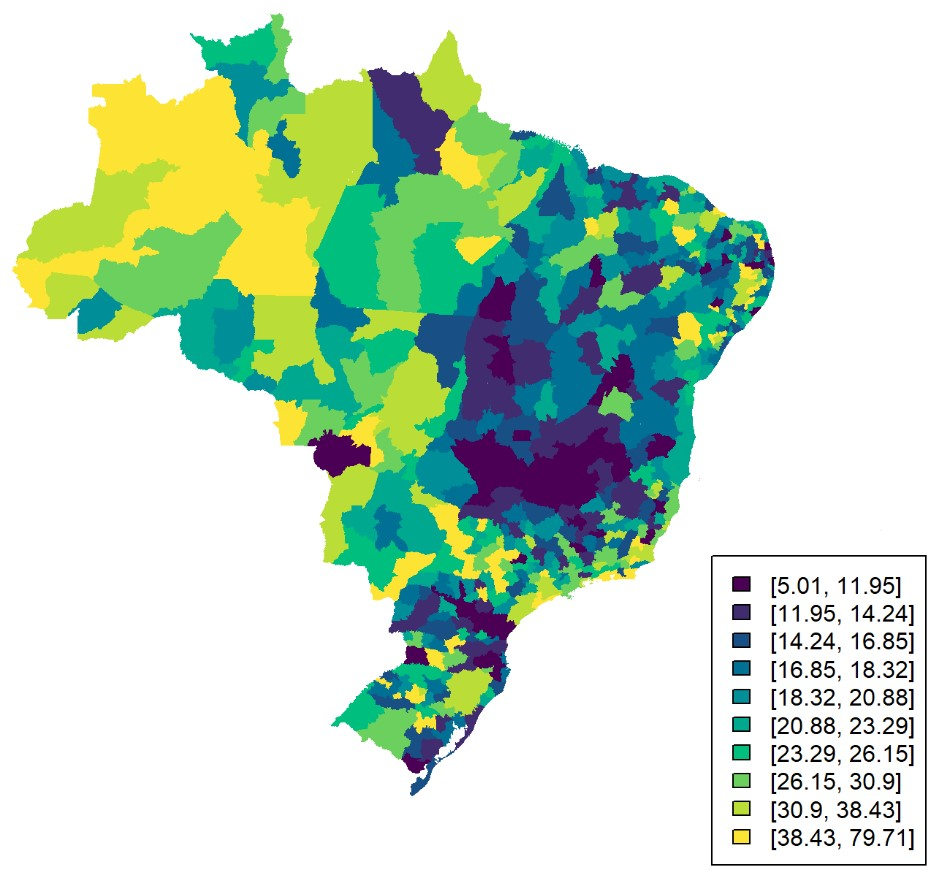
\includegraphics[scale=0.5]{pred_TB_rate_map.jpg} }}%
    \qquad
    \subfloat[\centering label 2]{{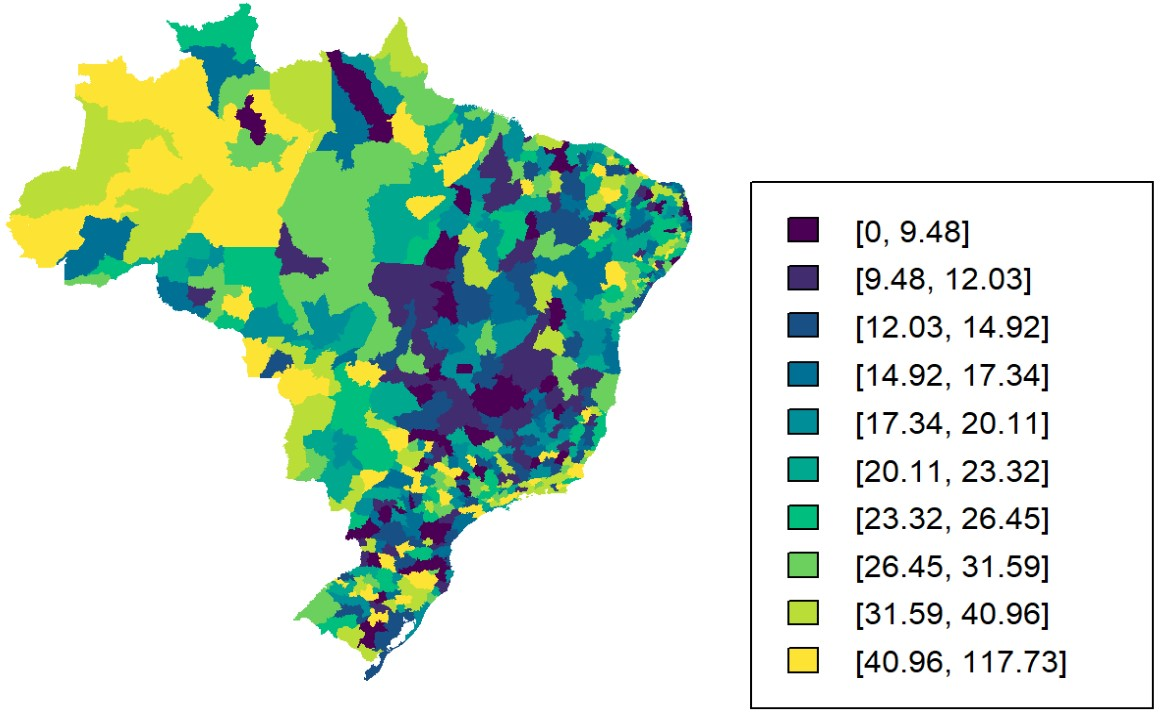
\includegraphics[scale=0.5]{true_TB_rate_map.jpg} }}%
    \caption{Predicted (a) and True(b) rates of TB per 100k inhabitants}%
    \label{fig:example}%
\end{figure}

\section{Critical Review}
Drawbacks of the Model:
\\
1. Predictions do not cover full range of data, as evinced by deviations in the QQ plot
\\
2. ??

\section{References}
Wood, S. N. (2017). Generalized Additive Models: An Introduction with R (2nd ed.). CRC Press.
\section{Appendix}

\subsection{Figures}

\begin{figure}[H]
\centering
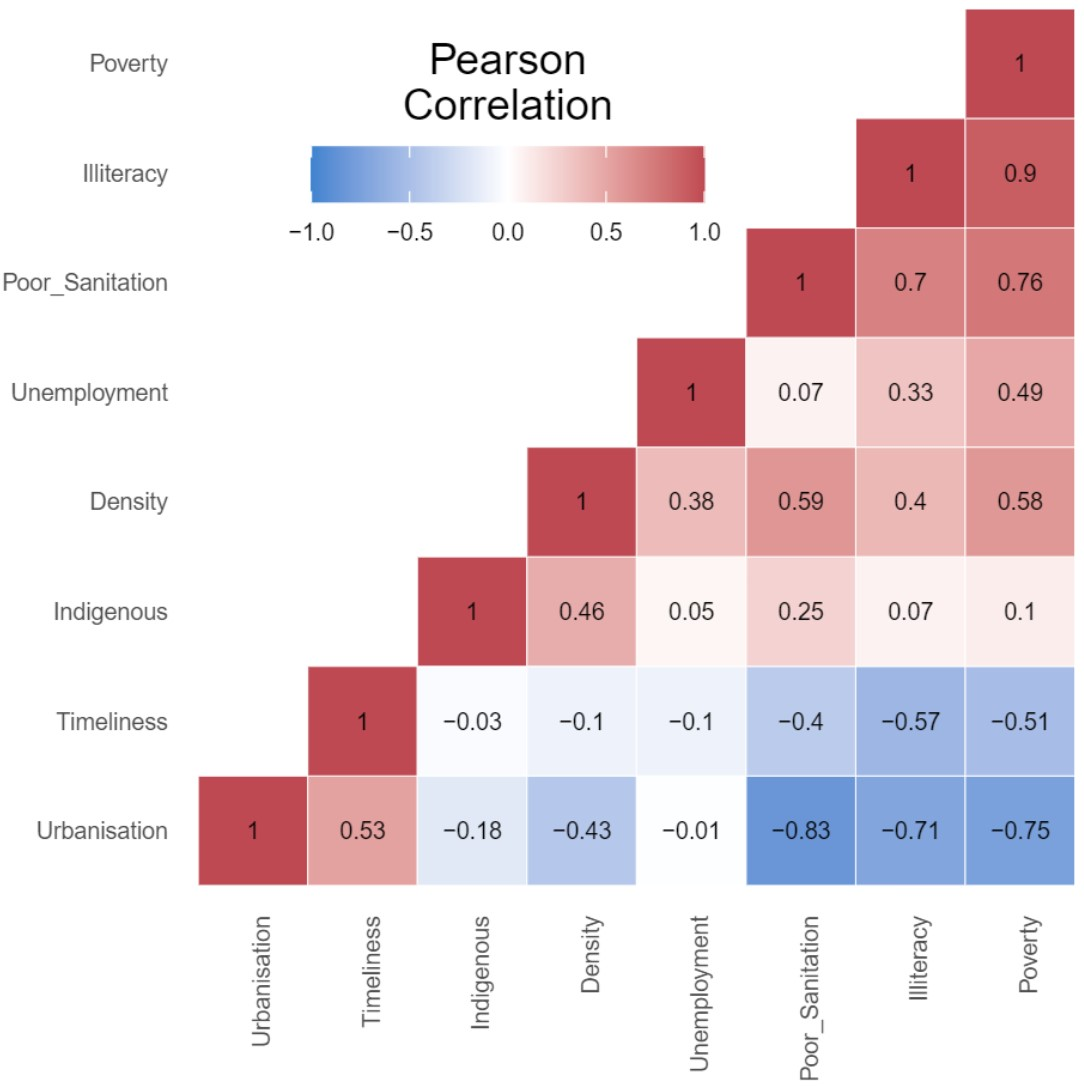
\includegraphics[scale=0.5]{pearson_correl.jpg}
\caption{\label{fig:pearson_correl}Correlogram shows covariates with highest positive and negative correlations.}
\end{figure}

\subsection{Tables}

\begin{table}[H]
\centering
\begin{tabular}{l|r}
Item & Quantity \\\hline
Widgets & 42 \\
Gadgets & 13
\end{tabular}
\caption{\label{tab:widgets}An example table.}
\end{table}

\subsection{Code}
\begin{verbatim}
#####################SS CODE######################
# Import Libraries
library(mgcv) # required for GAM 
library(tidyverse) 
library(ggplot2) # required for plotting
library(dplyr) # required for filtering dataset
library(fields) # required for maps
library(maps) # required for maps
library(reshape2) # only required for melt in corr plot
library(car) # only required for VIF

# Load Data
load("C:/Users/soura/Documents/COMM511/group_coursework/datasets_project.RData")

# Investigate correlation
### Resource -> http://www.sthda.com/english/wiki/ggplot2-quick-
### correlation-matrix-heatmap-r-software-and-data-visualization
cormat <- cor(TBdata[,c(1,2,3,4,5,6,7,8)])
# Reorder
reorder_cormat <- function(cormat){
  # Use correlation between variables as distance
  dd <- as.dist((1-cormat)/2)
  hc <- hclust(dd)
  cormat <-cormat[hc$order, hc$order]
}

# Reorder the correlation matrix
cormat <- reorder_cormat(cormat)
# Get lower triangular matrix
cormat[lower.tri(cormat)] <- NA

melted_cormat <- melt(cormat , na.rm = TRUE)
melted_cormat$value = round(melted_cormat$value, 2)

# Create a ggheatmap
ggheatmap <- ggplot(melted_cormat, aes(Var2, Var1, fill = value))+
 geom_tile(color = "white")+
 scale_fill_gradient2(low = "#1a85d6", high = "#cf3e4f", mid = "white", 
   midpoint = 0, limit = c(-1,1), space = "Lab", 
    name="Pearson\nCorrelation") +
  theme_minimal()+ # minimal theme
 theme(axis.text.x = element_text(angle = 90, vjust = 1, 
    size = 12, hjust = 1))+
 coord_fixed()

# Add correlation coefficients
ggheatmap +
geom_text(aes(Var2, Var1, label = value), color = "black", size = 2) +
theme(
  axis.text.x = element_text(size = 6),
  axis.text.y = element_text(size = 6),
  axis.title.x = element_blank(),
  axis.title.y = element_blank(),
  panel.grid.major = element_blank(),
  panel.border = element_blank(),
  panel.background = element_blank(),
  axis.ticks = element_blank(),
  legend.justification = c(1, 0),
  legend.position = c(0.6, 0.7),
  legend.direction = "horizontal",
  legend.text = element_text(size = 6)
  ) + 
  guides(fill = guide_colorbar(barwidth = 7, barheight = 1,
                title.position = "top", title.hjust = 0.5))

#### Illiteracy is highly correlated with Poverty
#### Carry out a Variance Inflation Test
model_all <- lm(TB ~ . , data = select(TBdata, 'Indigenous' , 'Illiteracy' , 
'Urbanisation' , 'Density' , 'Poverty', 'Unemployment' , 'Timeliness' , 'Year' ,
'TB' , 'Population'))  # with all the independent variables

vif(model_all) # Several variables are highly correlated

model_no_illiteracy <- lm(TB ~ . , data = select(TBdata, 'Indigenous', 
'Urbanisation' , 'Density' , 'Poverty', 'Unemployment' , 'Timeliness' , 'Year' ,
'TB' , 'Population'))  # with all the independent variables

vif(model_no_illiteracy) # Poverty and Unemployment still seem highly correlated

model_no_illiteracy_no_poverty <- lm(TB ~ . , data = select(TBdata, 'Indigenous', 
'Urbanisation' , 'Density', 'Unemployment' , 'Timeliness' , 'Year' ,
'TB' , 'Population'))  # with all the independent variables

vif(model_no_illiteracy_no_poverty) # almost no variable is highly correlated

## More formal tests are conducted to confirm the dropping of Illiteracy.
## Check to see if Poverty should be dropped as well
prelim.model.1 <- gam(formula = TB ~ offset(log(Population)) + s(Indigenous) + 
s(Illiteracy) + s(Urbanisation) + s(Density) + s(Poverty) + s(Poor_Sanitation)
+ s(Unemployment) + s(Timeliness),
data = TBdata , 
family = nb(link = 'log')
)
# Show summary
summary(prelim.model.1)
par(mfrow=c(2,2))
gam.check(prelim.model.1)

### Only the effect of illiteracy cannot be reliably stated to be non-zero
prelim.model.2 <- gam(formula = TB ~ offset(log(Population)) + s(Indigenous) 
+ s(Urbanisation) + s(Density) + s(Poverty) + s(Poor_Sanitation)
+ s(Unemployment) + s(Timeliness),
data = TBdata , 
family = nb(link = 'log')
)
# Show summary
summary(prelim.model.2)

# Show summary
summary(prelim.model.2)
par(mfrow=c(2,2))
gam.check(prelim.model.2)

# Likelihood ratio test
anova(prelim.model.1 , prelim.model.2 , test = 'F') # p-value is over 0.05
# The models are statistically indistinguishable

### Only the effect of illiteracy cannot be reliably stated to be non-zero
prelim.model.3 <- gam(formula = TB ~ offset(log(Population)) + s(Indigenous) 
+ s(Urbanisation) + s(Density) + s(Poor_Sanitation) + s(Unemployment) 
+ s(Timeliness),
data = TBdata , 
family = nb(link = 'log')
)
# Show summary
summary(prelim.model.3)

# Likelihood ratio test
anova(prelim.model.2 , prelim.model.3 , test = 'F') # p-value is less than 0.05
# The models are statistically different. Poverty should not be excluded.

### Model chosen (with social covariates) is the negative binomial without
### Illiteracy
summary(prelim.model.2) # Only 44% of the deviance is explained. Adding temporal
# and spatial covariates may improve this
par(mfrow=c(2,2))
gam.check(prelim.model.2)
par(mfrow = c(1,1))

### Only the effect of illiteracy cannot be reliably stated to be non-zero
prelim.model.4 <- gam(formula = TB ~ offset(log(Population)) + s(Indigenous , k = 20) 
+ s(Urbanisation , k = 20) + s(Density , k = 20) + s(Poverty , k = 20)
+ s(Poor_Sanitation , k = 20) + s(Unemployment , k = 20) + s(Timeliness , k = 20),
data = TBdata , 
family = nb(link = 'log')
)
# Show summary
summary(prelim.model.4)
par(mfrow=c(2,2))
gam.check(prelim.model.4)


### Adding spatial covariates
spatial.model <- gam(formula = TB ~ offset(log(Population)) + s(Indigenous) 
+ s(Urbanisation) + s(Density) + s(Poor_Sanitation) + s(Unemployment) +s(Poverty)
+ s(Timeliness) + s(lon , lat),
data = TBdata , 
family = nb(link = 'log')
)
# Check summary
summary(spatial.model)
# Check the smooth functions of the covars
plot(spatial.model)
par(mfrow=c(2,2))
gam.check(spatial.model)
par(mfrow = c(1,1))
spatial.model$aic

### Using separate smoothers
spatial.model.2 <- gam(formula = TB ~ offset(log(Population)) + s(Indigenous) 
+ s(Urbanisation) + s(Density) + s(Poor_Sanitation) + s(Unemployment) + s(Poverty)
+ s(Timeliness) + te(lon , lat , k = 20),
data = TBdata , 
family = nb(link = 'log')
)
# Check summary
summary(spatial.model.2)
# Check the smooth functions of the covariates
plot(spatial.model.2)
par(mfrow=c(2,2))
gam.check(spatial.model.2 , pch = 20)
par(mfrow = c(1,1))

### PREDICTIONS
fitted_nb <- predict(spatial.model.2, newdata = TBdata , type = 'response')

# PLOTTING STUFF - ERROR WHILE COMPILING - WILL FIX LATER
par(mfrow = c(1,1))
plot.map(exp(log(fitted_nb) - log(TBdata$Population))*100000 , n.levels = 10)


TBdata$Year.asFactor <- factor(TBdata$Year)

#### Temporal covariates
temporal.model <- gam(formula = TB ~ offset(log(Population)) + s(Indigenous) 
+ s(Urbanisation) + s(Density) + s(Poor_Sanitation) + s(Unemployment) + s(Poverty)
+ s(Timeliness) + Year.asFactor,
data = TBdata , 
family = nb(link = 'log')
)
# Check summary
summary(temporal.model) # Temporal alone doesn't add much to explaining the variance
# Check the smooth functions of the covariates
plot(temporal.model)
par(mfrow=c(2,2))
gam.check(temporal.model)
par(mfrow = c(1,1))

#### Temporal covariates
temporal.model.2 <- gam(formula = TB ~ offset(log(Population))
+ s(Indigenous , by=Year.asFactor) + s(Urbanisation , by=Year.asFactor)
+ s(Density , by=Year.asFactor) + s(Poor_Sanitation , by=Year.asFactor)
+ s(Unemployment , by=Year.asFactor) + s(Poverty , by=Year.asFactor)
+ s(Timeliness , by=Year.asFactor) , 
data = TBdata , 
family = nb(link = 'log')
)
# Check summary
summary(temporal.model.2) # Temporal alone doesn't add much to explaining the variance
# Check the smooth functions of the covariates
plot(temporal.model.2)
par(mfrow=c(2,2))
gam.check(temporal.model.2)
par(mfrow = c(1,1))

### Spatio-temporal model
spatio.temporal.model <- gam(formula = TB ~ offset(log(Population)) + s(Indigenous) 
+ s(Urbanisation) + s(Density) + s(Poor_Sanitation) + s(Unemployment) + s(Poverty)
+ s(Timeliness) + te(lon , lat , k = 20) + Year.asFactor,
data = TBdata , 
family = nb(link = 'log')
)
# Check summary
summary(spatio.temporal.model) # Temporal alone doesn't add much to explaining the variance
# Check the smooth functions of the covariates
plot(spatio.temporal.model)
par(mfrow=c(2,2))
gam.check(spatio.temporal.model , pch = 20)
par(mfrow = c(1,1))

# PLOT
fitted_nb <- predict(spatio.temporal.model, newdata = TBdata , type = 'response')
TBdata$pred_rate <- fitted_nb/TBdata$Population*100000

# PLOTTING STUFF - ERROR WHILE COMPILING - WILL FIX LATER
par(mfrow = c(1,1))
plot.map(TBdata$pred_rate , n.levels = 10)

### WIHTOUT POVERTY
### Spatio-temporal model - Poverty
spatio.temporal.model.wo.pov <- gam(formula = TB ~ offset(log(Population)) + s(Indigenous) 
+ s(Urbanisation) + s(Density) + s(Poor_Sanitation) + s(Unemployment)
+ s(Timeliness) + te(lon , lat , k = 20) + Year.asFactor,
data = TBdata , 
family = nb(link = 'log')
)

# Check summary
summary(spatio.temporal.model.wo.pov) # Temporal alone doesn't add much to explaining the variance
# Check the smooth functions of the covariates
plot(spatio.temporal.model.wo.pov)
par(mfrow=c(2,2))
gam.check(spatio.temporal.model.wo.pov , pch = 20)
par(mfrow = c(1,1))

# Anova test
anova(spatio.temporal.model.wo.pov , spatio.temporal.model , test = 'F')

### Without Indigenous
spatio.temporal.model.wo.indig <- gam(formula = TB ~ offset(log(Population))
+ s(Urbanisation) + s(Density) + s(Poor_Sanitation) + s(Unemployment) + s(Poverty)
+ s(Timeliness) + te(lon , lat , k = 20) + Year.asFactor,
data = TBdata , 
family = nb(link = 'log')
)

# Check summary
summary(spatio.temporal.model.wo.indig) # Temporal alone doesn't add much to explaining the variance
# Check the smooth functions of the covariates
plot(spatio.temporal.model.wo.indig)
par(mfrow=c(2,2))
gam.check(spatio.temporal.model.wo.indig , pch = 20)
par(mfrow = c(1,1))

# Anova test
anova(spatio.temporal.model.wo.indig , spatio.temporal.model , test = 'F')
# NOT ENOUGH EVIDENCE TO REMOVE INDIGENOUS

## Spatio-temporal model
spatio.temporal.model.true <- gam(formula = TB ~ offset(log(Population)) + s(Indigenous) 
+ s(Urbanisation) + s(Density) + s(Poor_Sanitation) + s(Unemployment) + s(Poverty)
+ s(Timeliness) + te(lon , lat , Year , k = 3),
data = TBdata , 
family = nb(link = 'log')
)

# Check summary
summary(spatio.temporal.model.true) # Temporal alone doesn't add much to explaining the variance
# Check the smooth functions of the covariates
plot(spatio.temporal.model.true)
par(mfrow=c(2,2))
gam.check(spatio.temporal.model.true , pch = 20)
par(mfrow = c(1,1))

spatio.temporal.model$aic
spatio.temporal.model.true$aic
spatio.temporal.model.wo.indig$aic



### Spatio-temporal model - no poor sanitation , indigenous
spatio.temporal.model.wo.indig.poor_s <- gam(formula = TB ~ offset(log(Population))
+ s(Urbanisation) + s(Density) + s(Unemployment) + s(Poverty)
+ s(Timeliness) + te(lon , lat , k = 20) + Year.asFactor,
data = TBdata , 
family = nb(link = 'log')
)
# Check summary
summary(spatio.temporal.model.wo.indig.poor_s) # Temporal alone doesn't add much to explaining the variance
# Check the smooth functions of the covariates
plot(spatio.temporal.model.wo.indig.poor_s)
par(mfrow=c(2,2))
gam.check(spatio.temporal.model.wo.indig.poor_s , pch = 20)
par(mfrow = c(1,1))

anova(spatio.temporal.model , spatio.temporal.model.wo.indig.poor_s , spatio.temporal.model.wo.indig , test = 'F')

################LH CODE############################################
library (mgcv)


par(mfrow = c(2,2))
#fit poisson model with socio-economic variables
model_poisson <- gam(formula = TB ~ offset(log(Population)) + s(Indigenous) +  s(Illiteracy) +  s(Urbanisation) + s(Density) + s(Poverty) + s(Poor_Sanitation) + s(Unemployment) + s(Timeliness), data = TBdata, family = poisson(link = 'log'))
summary(model_poisson)
model_poisson$aic
par(mfrow = c(2,2),pch = 20)
gam.check(model_poisson)
# #add flexibility
model_poisson <- gam(formula = TB ~ offset(log(Population)) + s(Indigenous, k = 80) +  s(Illiteracy, k = 80) +  s(Urbanisation, k = 80) + s(Density, k = 80) + s(Poverty, k = 80) + s(Poor_Sanitation, k = 80) + s(Unemployment, k = 80) + s(Timeliness, k = 80), data = TBdata, family = poisson(link = 'log'))
gam.check(model_poisson)
summary(model_poisson) # SIGNS OF OVERFIT
plot(model_poisson) # SIGNS OF OVERFIT
#fit negative binomial model with  socioeconomic
model_nb <- gam(formula = TB ~ offset(log(Population)) + s(Indigenous) +  s(Illiteracy) + s(Urbanisation) + s(Density) + s(Poverty) + s(Poor_Sanitation) + s(Unemployment) + s(Timeliness), data = TBdata, family = nb(link = 'log'))
summary(model_nb)
model_nb$aic
#fit a linear relation between sqaured residuals and prediction to see whether another model describes the variance-fitted values relation better
summary(lm(log(model_nb$residuals^2) ~ log(predict(model_nb, type = 'response'))))
#drop Illiteracy
model_nb_2 <- gam(formula = TB ~ offset(log(Population)) + s(Indigenous) +  s(Urbanisation) + s(Density) + s(Poverty) + s(Poor_Sanitation) + s(Unemployment) + s(Timeliness), data = TBdata, family = nb(link = 'log'))


#LRT
anova.gam(model_nb_2, model_nb, test = 'LRT')
#Null hypothesis not rejected -> drop poverty
model_nb_3 <- gam(formula = TB ~ offset(log(Population)) + s(Indigenous) +  s(Urbanisation) + s(Density) + s(Poor_Sanitation) + s(Unemployment) + s(Timeliness), data = TBdata, family = nb(link = 'log'))
#LRT
anova.gam(model_nb_3, model_nb_2, test = 'LRT')
# NULL hypothesis rejected -> drop only illiteracy, not poverty

model_nb_final <- model_nb_2
summary(model_nb_final)
gam.check(model_nb_final)
fitted_nb <- predict(model_nb_final, type = 'response')

# PLOTTING STUFF - ERROR WHILE COMPILING - WILL FIX LATER
par(mfrow = c(1,2))
plot.map(log(fitted_nb) - log(TBdata$Population) , n.levels = 10)
plot.map(log(TBdata$TB) - log(TBdata$Population))

#temporal model
par(mfrow = c(2,2), pch = 20)
model_nb_time <- gam(formula = TB ~ offset(log(Population)) + s(Indigenous, by = Year) + s(Urbanisation, by = Year) + s(Density, by = Year) + s(Poverty, by = Year) + s(Poor_Sanitation, by = Year) + s(Unemployment, by = Year) + s(Timeliness, by = Year), data = TBdata, family = nb(link = 'log'))
summary(model_nb)
model_nb$aic

#spatial model
model_nb_space <- gam(formula = TB ~ offset(log(Population)) + s(Indigenous) + s(Urbanisation) + s(Density) + s(Poverty) + s(Poor_Sanitation) + s(Unemployment) + s(Timeliness) + te(lon, lat), data = TBdata, family = nb(link = 'log'))
summary(model_nb_space)
model_nb_space$aic
gam.check(model_nb_space)
anova.gam(model_nb_space, model_nb_final, test = 'LRT')

#spatio-temporal model
model_nb_time_and_space <- gam(formula = TB ~ offset(log(Population)) + s(Urbanisation, by = Year) + s(Density, by = Year) + s(Poverty, by = Year) + s(Poor_Sanitation, by = Year) + s(Timeliness, by = Year) + s(Unemployment, by = Year) + te(lon,lat, by = Year), data = TBdata, family = nb(link = 'log'))
summary(model_nb_time_and_space)
model_nb_time_and_space$aic
gam.check(model_nb_time_and_space)

# PLOT
fitted_nb <- predict(model_nb_time_and_space, newdata = TBdata , type = 'response')

# PLOTTING STUFF - ERROR WHILE COMPILING - WILL FIX LATER
par(mfrow = c(1,1))
plot.map(exp(log(fitted_nb) - log(TBdata$Population))*100000 , n.levels = 10)
\end{verbatim}

\end{document}